% Options for packages loaded elsewhere
\PassOptionsToPackage{unicode}{hyperref}
\PassOptionsToPackage{hyphens}{url}
\PassOptionsToPackage{dvipsnames,svgnames,x11names}{xcolor}
%
\documentclass[
]{article}

\usepackage{amsmath,amssymb}
\usepackage{iftex}
\ifPDFTeX
  \usepackage[T1]{fontenc}
  \usepackage[utf8]{inputenc}
  \usepackage{textcomp} % provide euro and other symbols
\else % if luatex or xetex
  \usepackage{unicode-math}
  \defaultfontfeatures{Scale=MatchLowercase}
  \defaultfontfeatures[\rmfamily]{Ligatures=TeX,Scale=1}
\fi
\usepackage{lmodern}
\ifPDFTeX\else  
    % xetex/luatex font selection
\fi
% Use upquote if available, for straight quotes in verbatim environments
\IfFileExists{upquote.sty}{\usepackage{upquote}}{}
\IfFileExists{microtype.sty}{% use microtype if available
  \usepackage[]{microtype}
  \UseMicrotypeSet[protrusion]{basicmath} % disable protrusion for tt fonts
}{}
\makeatletter
\@ifundefined{KOMAClassName}{% if non-KOMA class
  \IfFileExists{parskip.sty}{%
    \usepackage{parskip}
  }{% else
    \setlength{\parindent}{0pt}
    \setlength{\parskip}{6pt plus 2pt minus 1pt}}
}{% if KOMA class
  \KOMAoptions{parskip=half}}
\makeatother
\usepackage{xcolor}
\usepackage[margin=1in]{geometry}
\setlength{\emergencystretch}{3em} % prevent overfull lines
\setcounter{secnumdepth}{5}
% Make \paragraph and \subparagraph free-standing
\makeatletter
\ifx\paragraph\undefined\else
  \let\oldparagraph\paragraph
  \renewcommand{\paragraph}{
    \@ifstar
      \xxxParagraphStar
      \xxxParagraphNoStar
  }
  \newcommand{\xxxParagraphStar}[1]{\oldparagraph*{#1}\mbox{}}
  \newcommand{\xxxParagraphNoStar}[1]{\oldparagraph{#1}\mbox{}}
\fi
\ifx\subparagraph\undefined\else
  \let\oldsubparagraph\subparagraph
  \renewcommand{\subparagraph}{
    \@ifstar
      \xxxSubParagraphStar
      \xxxSubParagraphNoStar
  }
  \newcommand{\xxxSubParagraphStar}[1]{\oldsubparagraph*{#1}\mbox{}}
  \newcommand{\xxxSubParagraphNoStar}[1]{\oldsubparagraph{#1}\mbox{}}
\fi
\makeatother


\providecommand{\tightlist}{%
  \setlength{\itemsep}{0pt}\setlength{\parskip}{0pt}}\usepackage{longtable,booktabs,array}
\usepackage{calc} % for calculating minipage widths
% Correct order of tables after \paragraph or \subparagraph
\usepackage{etoolbox}
\makeatletter
\patchcmd\longtable{\par}{\if@noskipsec\mbox{}\fi\par}{}{}
\makeatother
% Allow footnotes in longtable head/foot
\IfFileExists{footnotehyper.sty}{\usepackage{footnotehyper}}{\usepackage{footnote}}
\makesavenoteenv{longtable}
\usepackage{graphicx}
\makeatletter
\def\maxwidth{\ifdim\Gin@nat@width>\linewidth\linewidth\else\Gin@nat@width\fi}
\def\maxheight{\ifdim\Gin@nat@height>\textheight\textheight\else\Gin@nat@height\fi}
\makeatother
% Scale images if necessary, so that they will not overflow the page
% margins by default, and it is still possible to overwrite the defaults
% using explicit options in \includegraphics[width, height, ...]{}
\setkeys{Gin}{width=\maxwidth,height=\maxheight,keepaspectratio}
% Set default figure placement to htbp
\makeatletter
\def\fps@figure{htbp}
\makeatother

\usepackage{graphicx}
\DeclareGraphicsExtensions{.png,.pdf,.jpg}
\usepackage{float}
\usepackage[section]{placeins}
\makeatletter
\@ifpackageloaded{tcolorbox}{}{\usepackage[skins,breakable]{tcolorbox}}
\@ifpackageloaded{fontawesome5}{}{\usepackage{fontawesome5}}
\definecolor{quarto-callout-color}{HTML}{909090}
\definecolor{quarto-callout-note-color}{HTML}{0758E5}
\definecolor{quarto-callout-important-color}{HTML}{CC1914}
\definecolor{quarto-callout-warning-color}{HTML}{EB9113}
\definecolor{quarto-callout-tip-color}{HTML}{00A047}
\definecolor{quarto-callout-caution-color}{HTML}{FC5300}
\definecolor{quarto-callout-color-frame}{HTML}{acacac}
\definecolor{quarto-callout-note-color-frame}{HTML}{4582ec}
\definecolor{quarto-callout-important-color-frame}{HTML}{d9534f}
\definecolor{quarto-callout-warning-color-frame}{HTML}{f0ad4e}
\definecolor{quarto-callout-tip-color-frame}{HTML}{02b875}
\definecolor{quarto-callout-caution-color-frame}{HTML}{fd7e14}
\makeatother
\makeatletter
\@ifpackageloaded{caption}{}{\usepackage{caption}}
\AtBeginDocument{%
\ifdefined\contentsname
  \renewcommand*\contentsname{Table of contents}
\else
  \newcommand\contentsname{Table of contents}
\fi
\ifdefined\listfigurename
  \renewcommand*\listfigurename{List of Figures}
\else
  \newcommand\listfigurename{List of Figures}
\fi
\ifdefined\listtablename
  \renewcommand*\listtablename{List of Tables}
\else
  \newcommand\listtablename{List of Tables}
\fi
\ifdefined\figurename
  \renewcommand*\figurename{Figure}
\else
  \newcommand\figurename{Figure}
\fi
\ifdefined\tablename
  \renewcommand*\tablename{Table}
\else
  \newcommand\tablename{Table}
\fi
}
\@ifpackageloaded{float}{}{\usepackage{float}}
\floatstyle{ruled}
\@ifundefined{c@chapter}{\newfloat{codelisting}{h}{lop}}{\newfloat{codelisting}{h}{lop}[chapter]}
\floatname{codelisting}{Listing}
\newcommand*\listoflistings{\listof{codelisting}{List of Listings}}
\makeatother
\makeatletter
\makeatother
\makeatletter
\@ifpackageloaded{caption}{}{\usepackage{caption}}
\@ifpackageloaded{subcaption}{}{\usepackage{subcaption}}
\makeatother

\ifLuaTeX
  \usepackage{selnolig}  % disable illegal ligatures
\fi
\usepackage{bookmark}

\IfFileExists{xurl.sty}{\usepackage{xurl}}{} % add URL line breaks if available
\urlstyle{same} % disable monospaced font for URLs
\hypersetup{
  pdftitle={Twitter and the Politics of the Federal Deficit},
  pdfauthor={Cy Coldiron},
  colorlinks=true,
  linkcolor={blue},
  filecolor={Maroon},
  citecolor={Blue},
  urlcolor={Blue},
  pdfcreator={LaTeX via pandoc}}


\title{Twitter and the Politics of the Federal Deficit}
\usepackage{etoolbox}
\makeatletter
\providecommand{\subtitle}[1]{% add subtitle to \maketitle
  \apptocmd{\@title}{\par {\large #1 \par}}{}{}
}
\makeatother
\subtitle{Results (Draft)}
\author{Cy Coldiron}
\date{2025-10-02}

\begin{document}
\maketitle

\renewcommand*\contentsname{Table of contents}
{
\hypersetup{linkcolor=}
\setcounter{tocdepth}{3}
\tableofcontents
}

\begin{tcolorbox}[enhanced jigsaw, breakable, bottomtitle=1mm, opacitybacktitle=0.6, left=2mm, rightrule=.15mm, title=\textcolor{quarto-callout-important-color}{\faExclamation}\hspace{0.5em}{Important}, coltitle=black, toptitle=1mm, colback=white, arc=.35mm, titlerule=0mm, bottomrule=.15mm, colframe=quarto-callout-important-color-frame, leftrule=.75mm, colbacktitle=quarto-callout-important-color!10!white, opacityback=0, toprule=.15mm]

\textbf{Writing sample disclaimer.} This PDF contains a draft of the
\emph{Results} section from the working paper\\
\textbf{Twitter and the Politics of the Federal Deficit}. The abstract
is included below for context.

\end{tcolorbox}

\subsection{Abstract (for context)}\label{abstract-for-context}

A long-held belief in American politics is that elected officials'
concern about the federal deficit is mainly a function of who holds
power. Amid deepening polarization, elevated public debt, and the shift
of political communication online, it is vital---for voters,
policymakers, and public-knowledge institutions---to understand
empirically how deficit rhetoric operates in these spaces. I analyze
\textasciitilde3.6 million tweets from official congressional accounts
(June 2017--January 2023), identify deficit-related posts using a
two-tier keyword approach, and estimate member--month logistic models
linked to leadership roles and legislative windows. My research confirms
that deficit rhetoric is rare but fluctuates greatly depending on two
contexts: relative institutional power (ie, minority / majority party),
and legislative periods (ie, Tax Cuts and Jobs Act, Inflation Reduction
Act). These findings contribute to understanding the modern incentive
structures and patterns of U.S. political communication strategies,
illustrating that deficit rhetoric is less a barometer of underlying
fiscal conditions than a tool used to serve political and partisan
interests.

\clearpage

\section{Macro Trends}\label{sec-macro}

\begin{figure}

\centering{

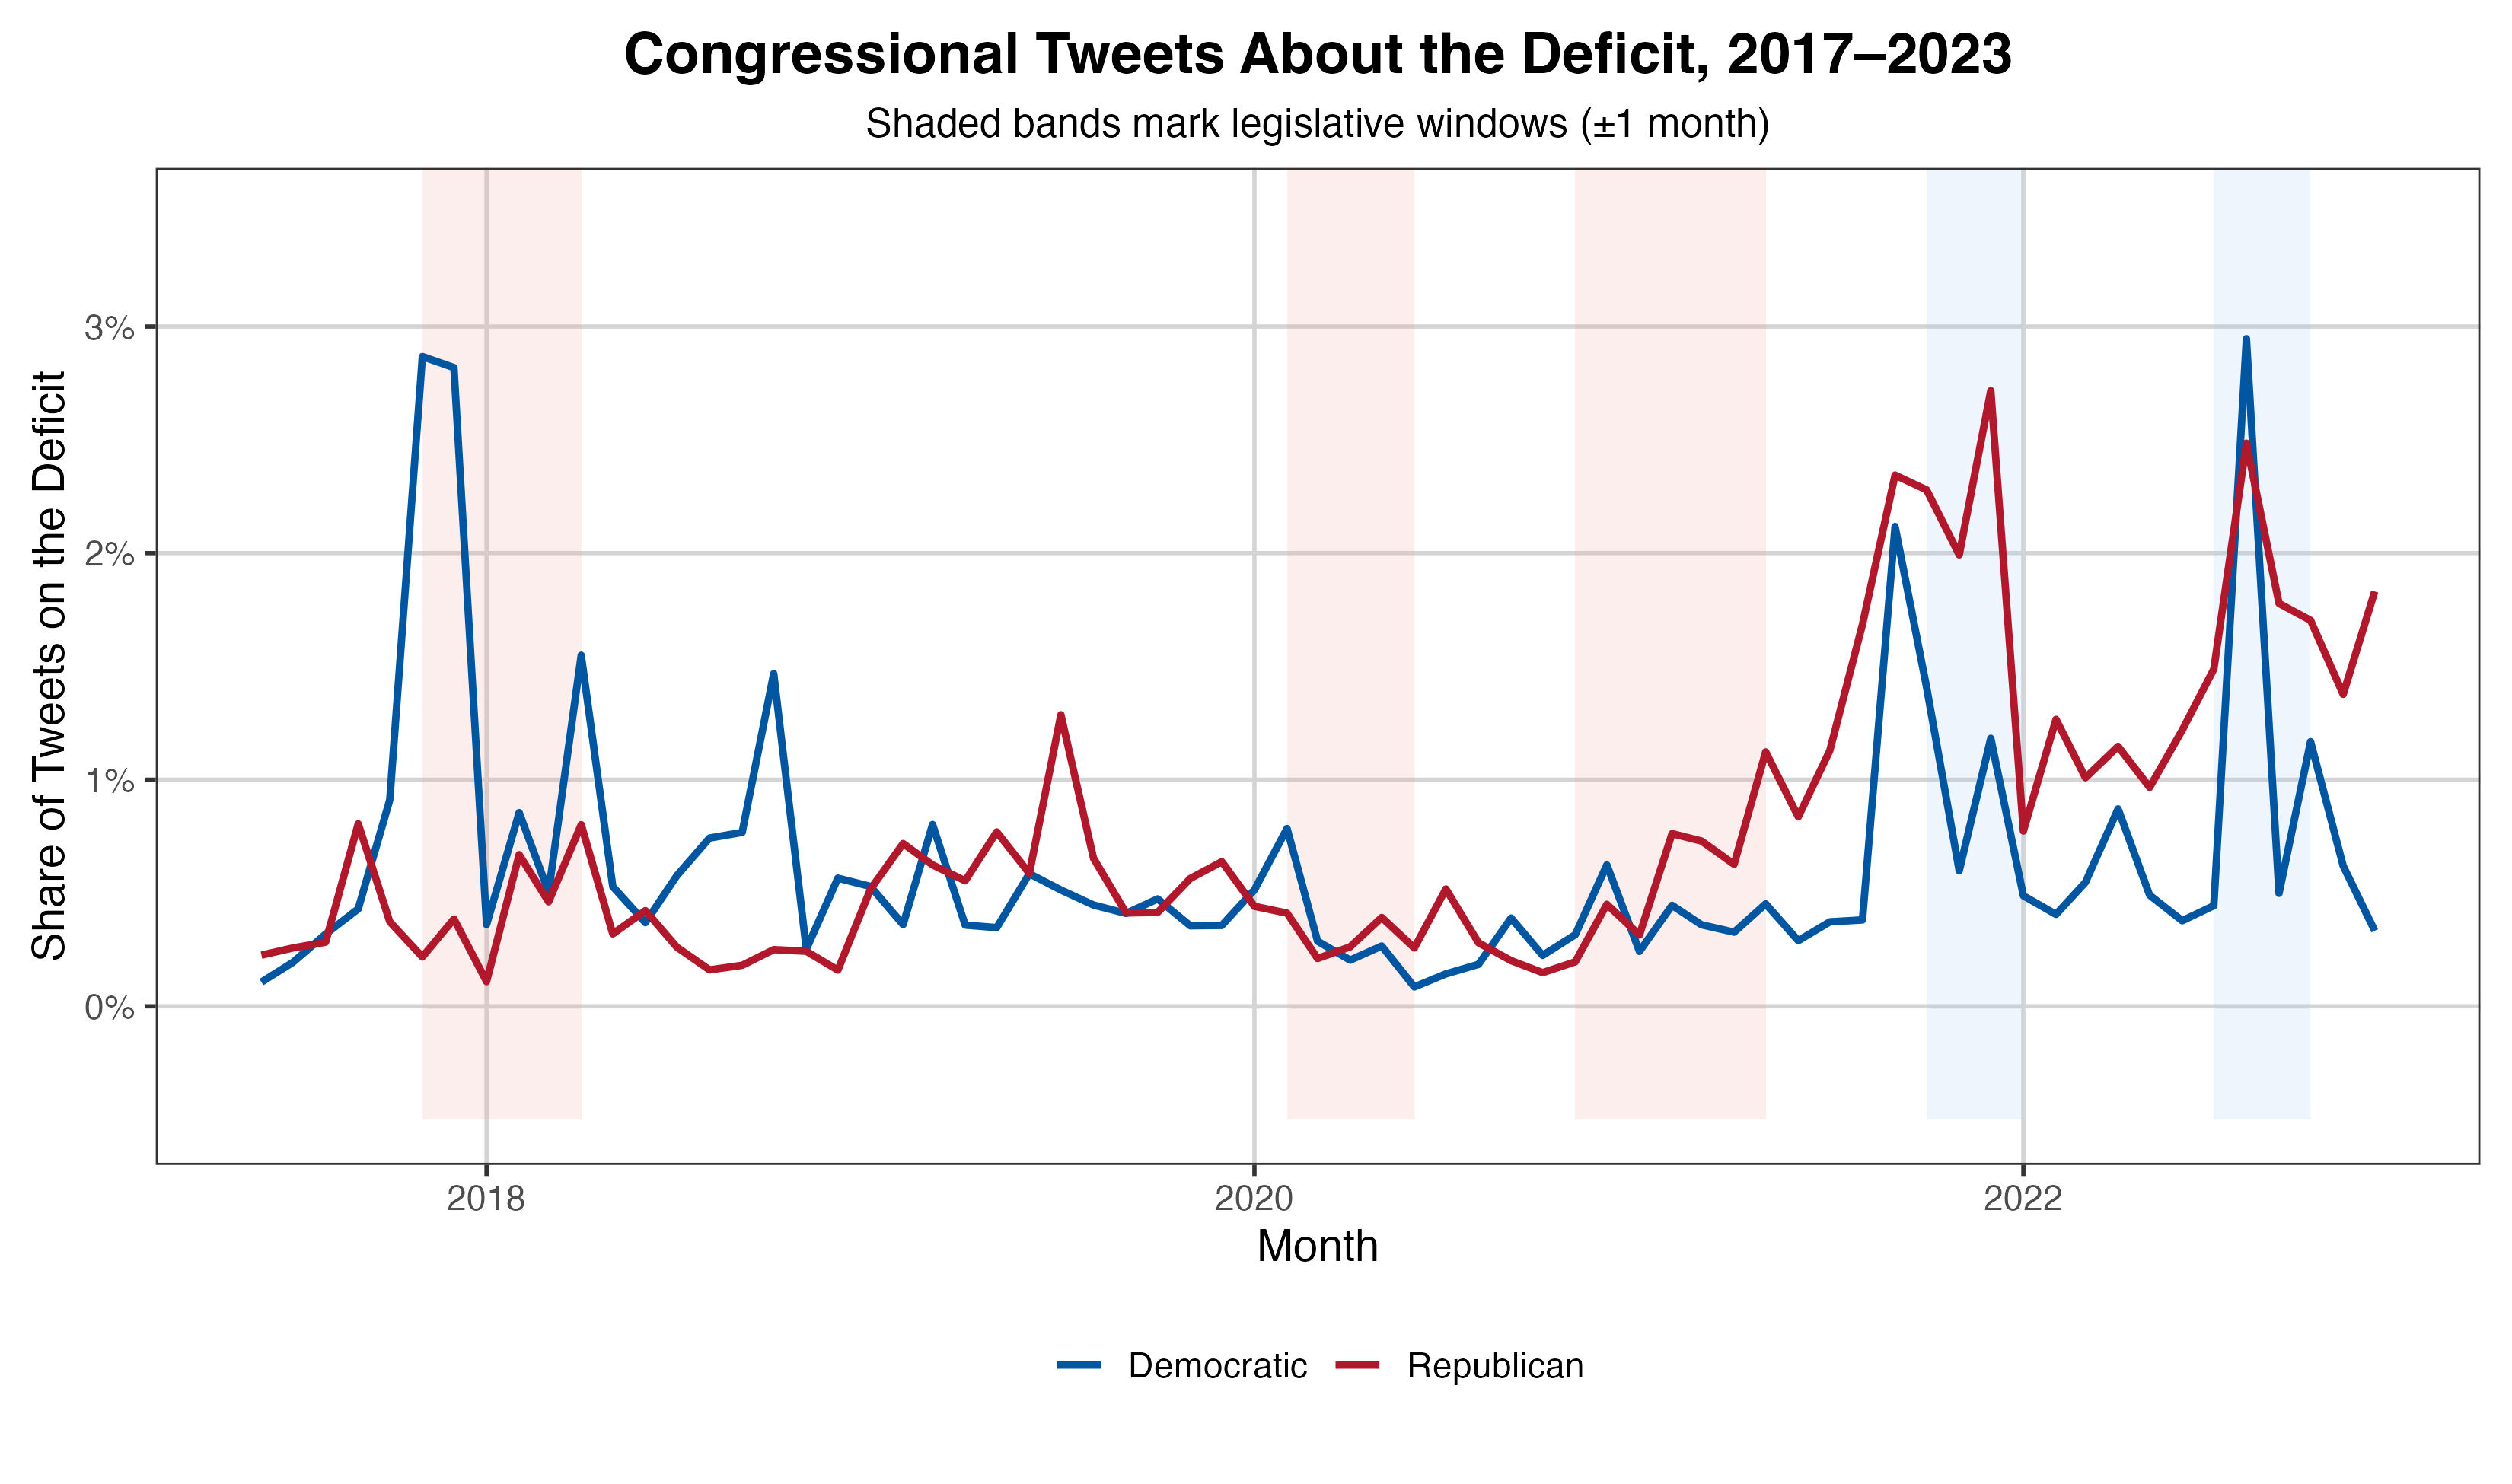
\includegraphics[width=0.85\textwidth,height=\textheight]{../figures/summary/deficit_tweet_share_with_legislation.png}

}

\caption{\label{fig-timeseries}Share of congressional tweets about the
deficit}

\end{figure}%

Figure~\ref{fig-timeseries} shows the monthly share of congressional
deficit tweets, by party, from June 2017 to January 2023. Consistent
with best practices in political science, this paper will represent the
Republican Party with red shading and the Democratic Party with blue.
Shaded areas indicate legislative periods -- defined as the month
before, during, and after the passage of a fiscally significant bill.
Legislative periods exclude small appropriations, procedural votes, and
commemorations.

The baseline deficit tweeting share for both parties is low, generally
staying under 1\% across the six years, with notable accelerations
occurring around legislative periods. Democratic tweeting patterns
remain relatively consistent across the six years, with three notable
peaks, all during legislative periods: December 2017 (Tax Cuts and Jobs
Act), October 2021 (Infrastructure Investment and Jobs Act), and August
2022 (Inflation Reduction Act, CHIPS \& Science Act). Republicans,
however, demonstrate consistently higher deficit tweeting rates as the
minority party, as illustrated in the peaks (2022, 2023) compared to
relatively low rates from 2017-2021.

\section{Economic Indicators}\label{economic-indicators}

\begin{figure}

\centering{

\includegraphics[width=0.85\textwidth,height=\textheight]{../figures/economic_indicators/g1_deficit_vs_approval_int_panel.png}

}

\caption{\label{fig-deficit-vs-indicators}Deficit tweet share vs 10-year
Treasury yield and congressional approval; rescaled.}

\end{figure}%

\begin{figure}

\centering{


\includegraphics[width=0.85\textwidth,height=\textheight]{../figures/economic_indicators/deficit_share_vs_inflation_smoothed.png}

}

\caption{\label{fig-deficit-vs-cpi}Deficit tweet share vs.~U.S. CPI
inflation.}

\end{figure}%

\FloatBarrier

Figure~\ref{fig-deficit-vs-indicators} plots deficit tweet share against
the 10-year Treasury yield and congressional approval, both rescaled for
comparability. The small correlation coefficients (0.44,~ -.07) suggest
no discernible linear relationship. In contrast,
Figure~\ref{fig-deficit-vs-cpi} -- which plots deficit tweeting against
US CPI inflation, reveals a relatively strong positive relationship, as
indicated by its large r-value (.78). We will explore several plausible
explanations for this correlation in the discussion section.

\section{Member-Level Patterns}\label{member-level-patterns}

\begin{figure}[H]

\centering{

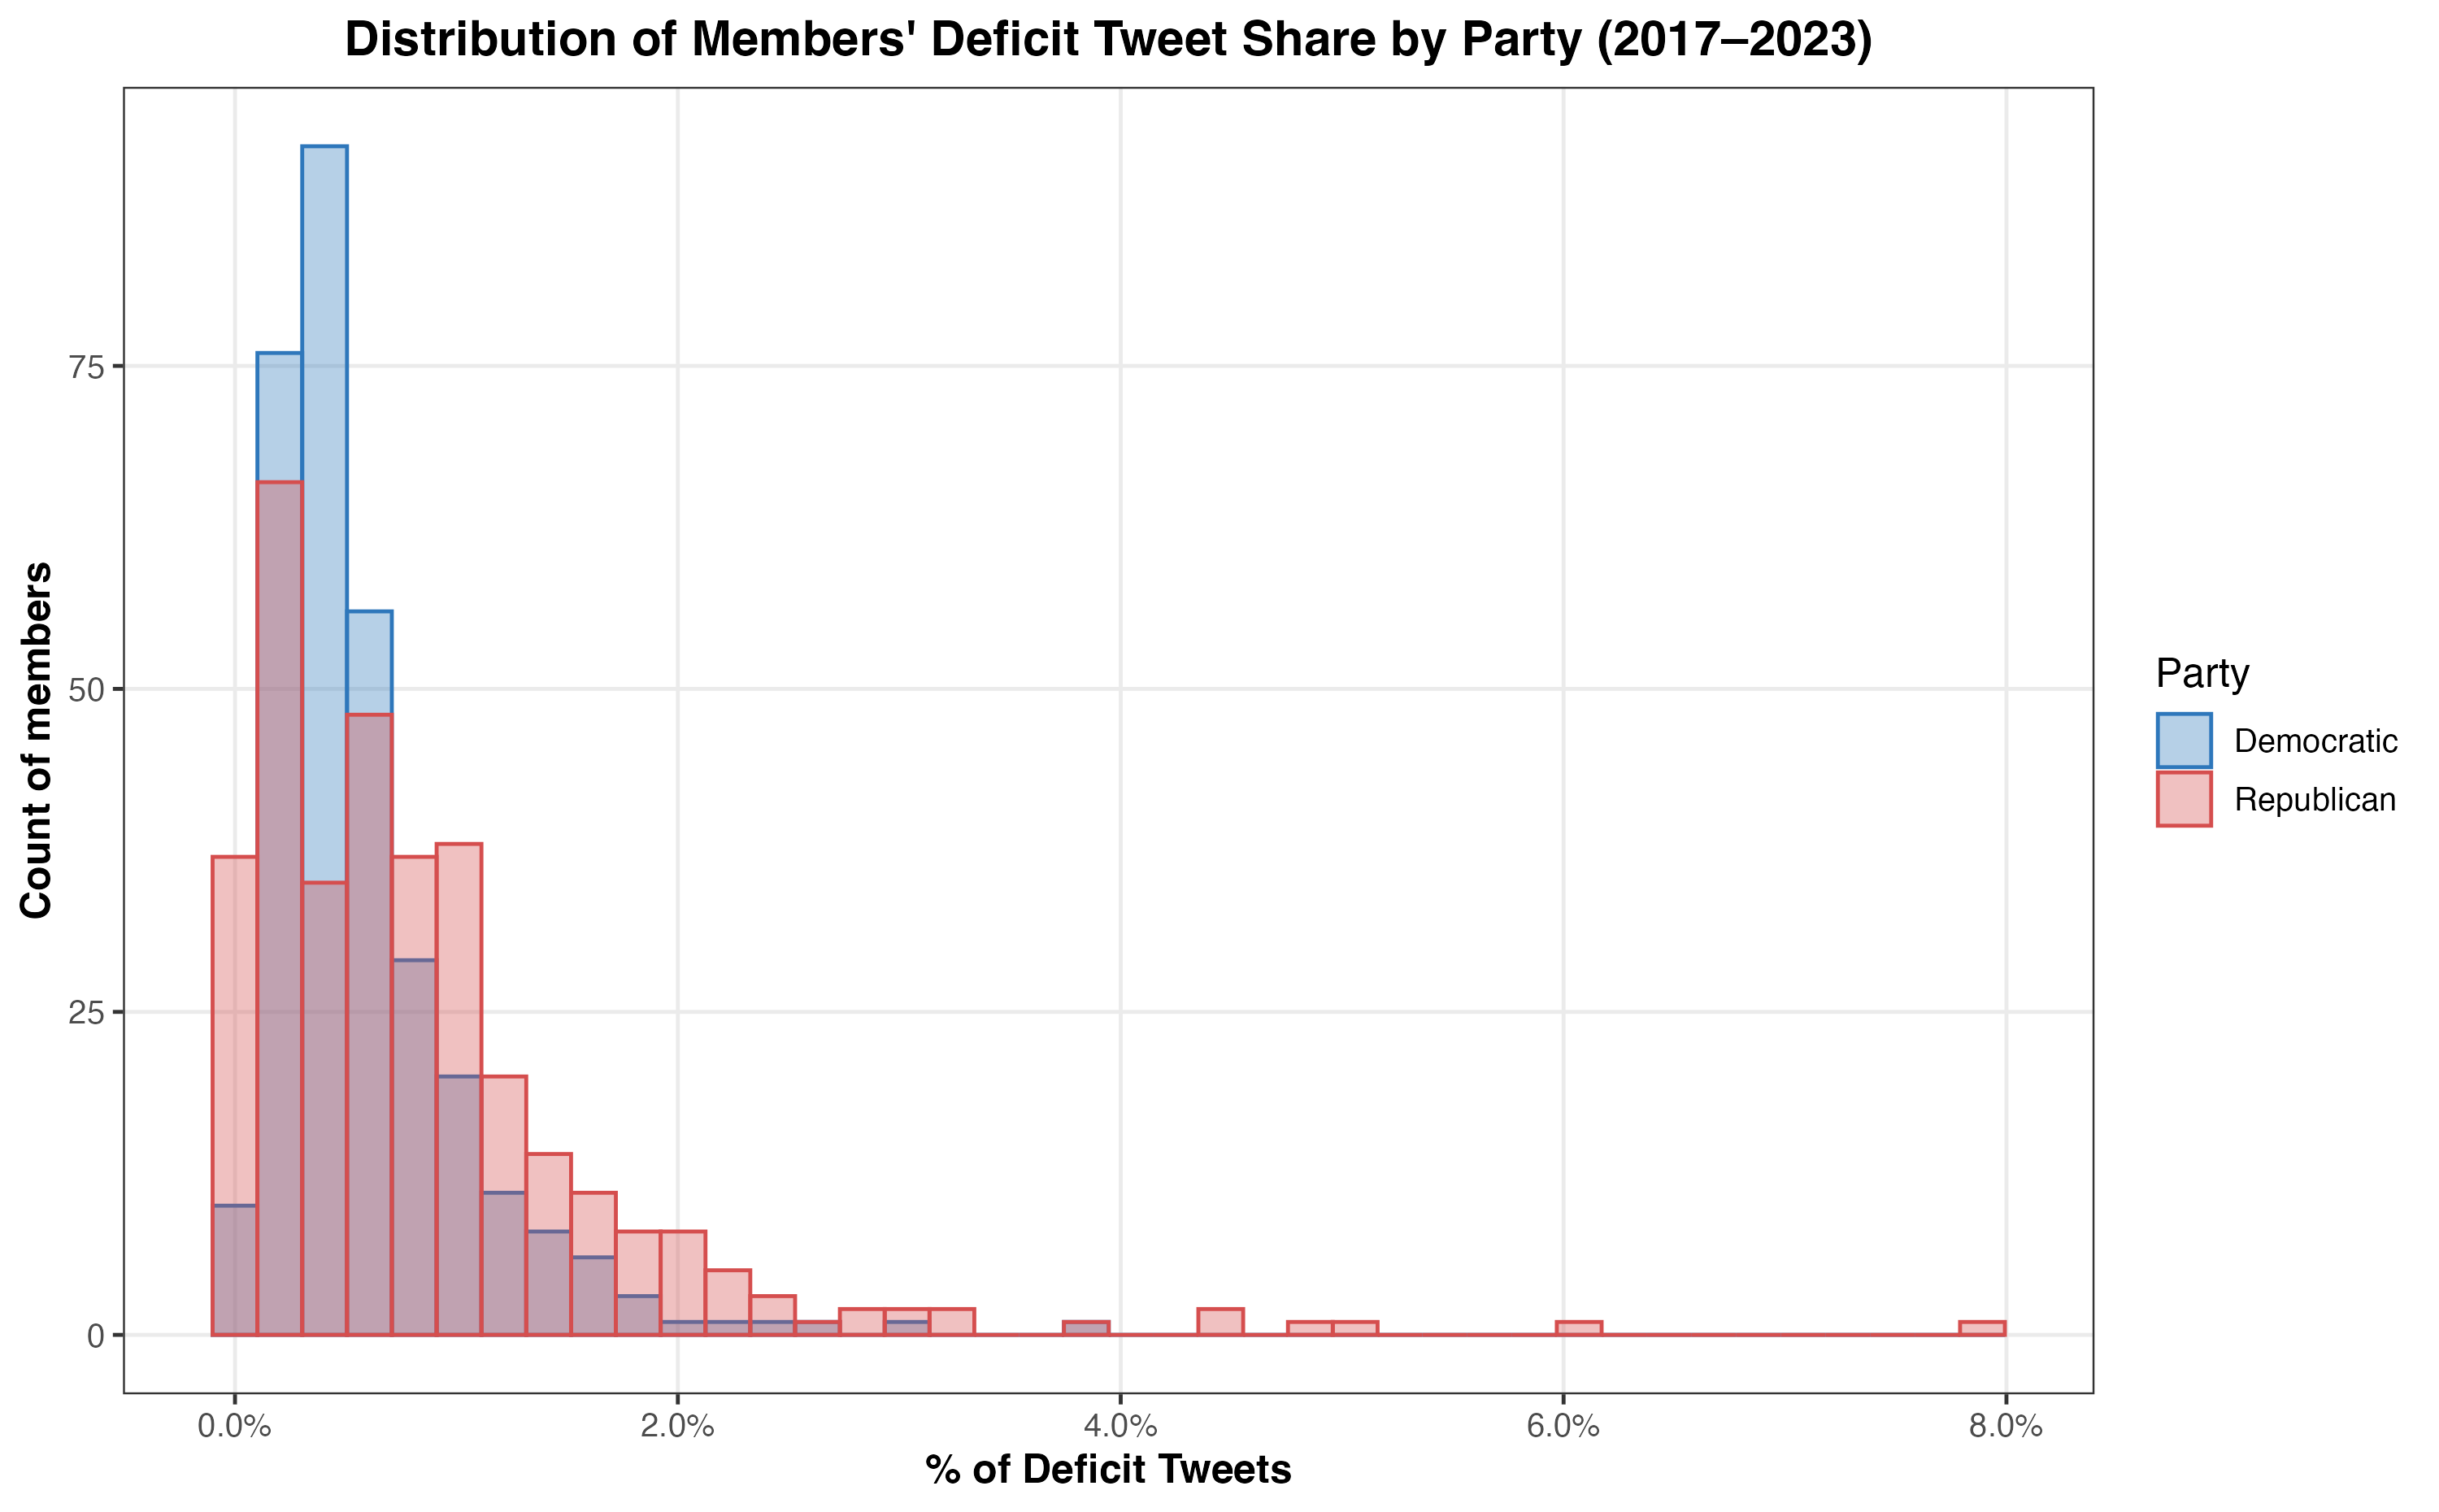
\includegraphics[width=0.75\textwidth,height=\textheight]{../figures/individuals/hist_pct_deficit_by_party.png}

}

\caption{\label{fig-member-share-by-party}Share of deficit tweets by
party (member-level distribution).}

\end{figure}%

\FloatBarrier

Deficit tweeting is uncommon across both Deficit tweeting is uncommon
across both parties, with the vast majority of members posting fewer
than \textbf{(1.5\%)} of their tweets on the deficit. Democrats display
a compact distribution: most fall below \textbf{(0.6\%)} with no
Democratic member exceeding \textbf{(2.5\%)}. Republicans show greater
variability, as illustrated by their distribution's long right tail,
which reaches \textbf{(4--8\%).}

\FloatBarrier

\begin{figure}

\centering{

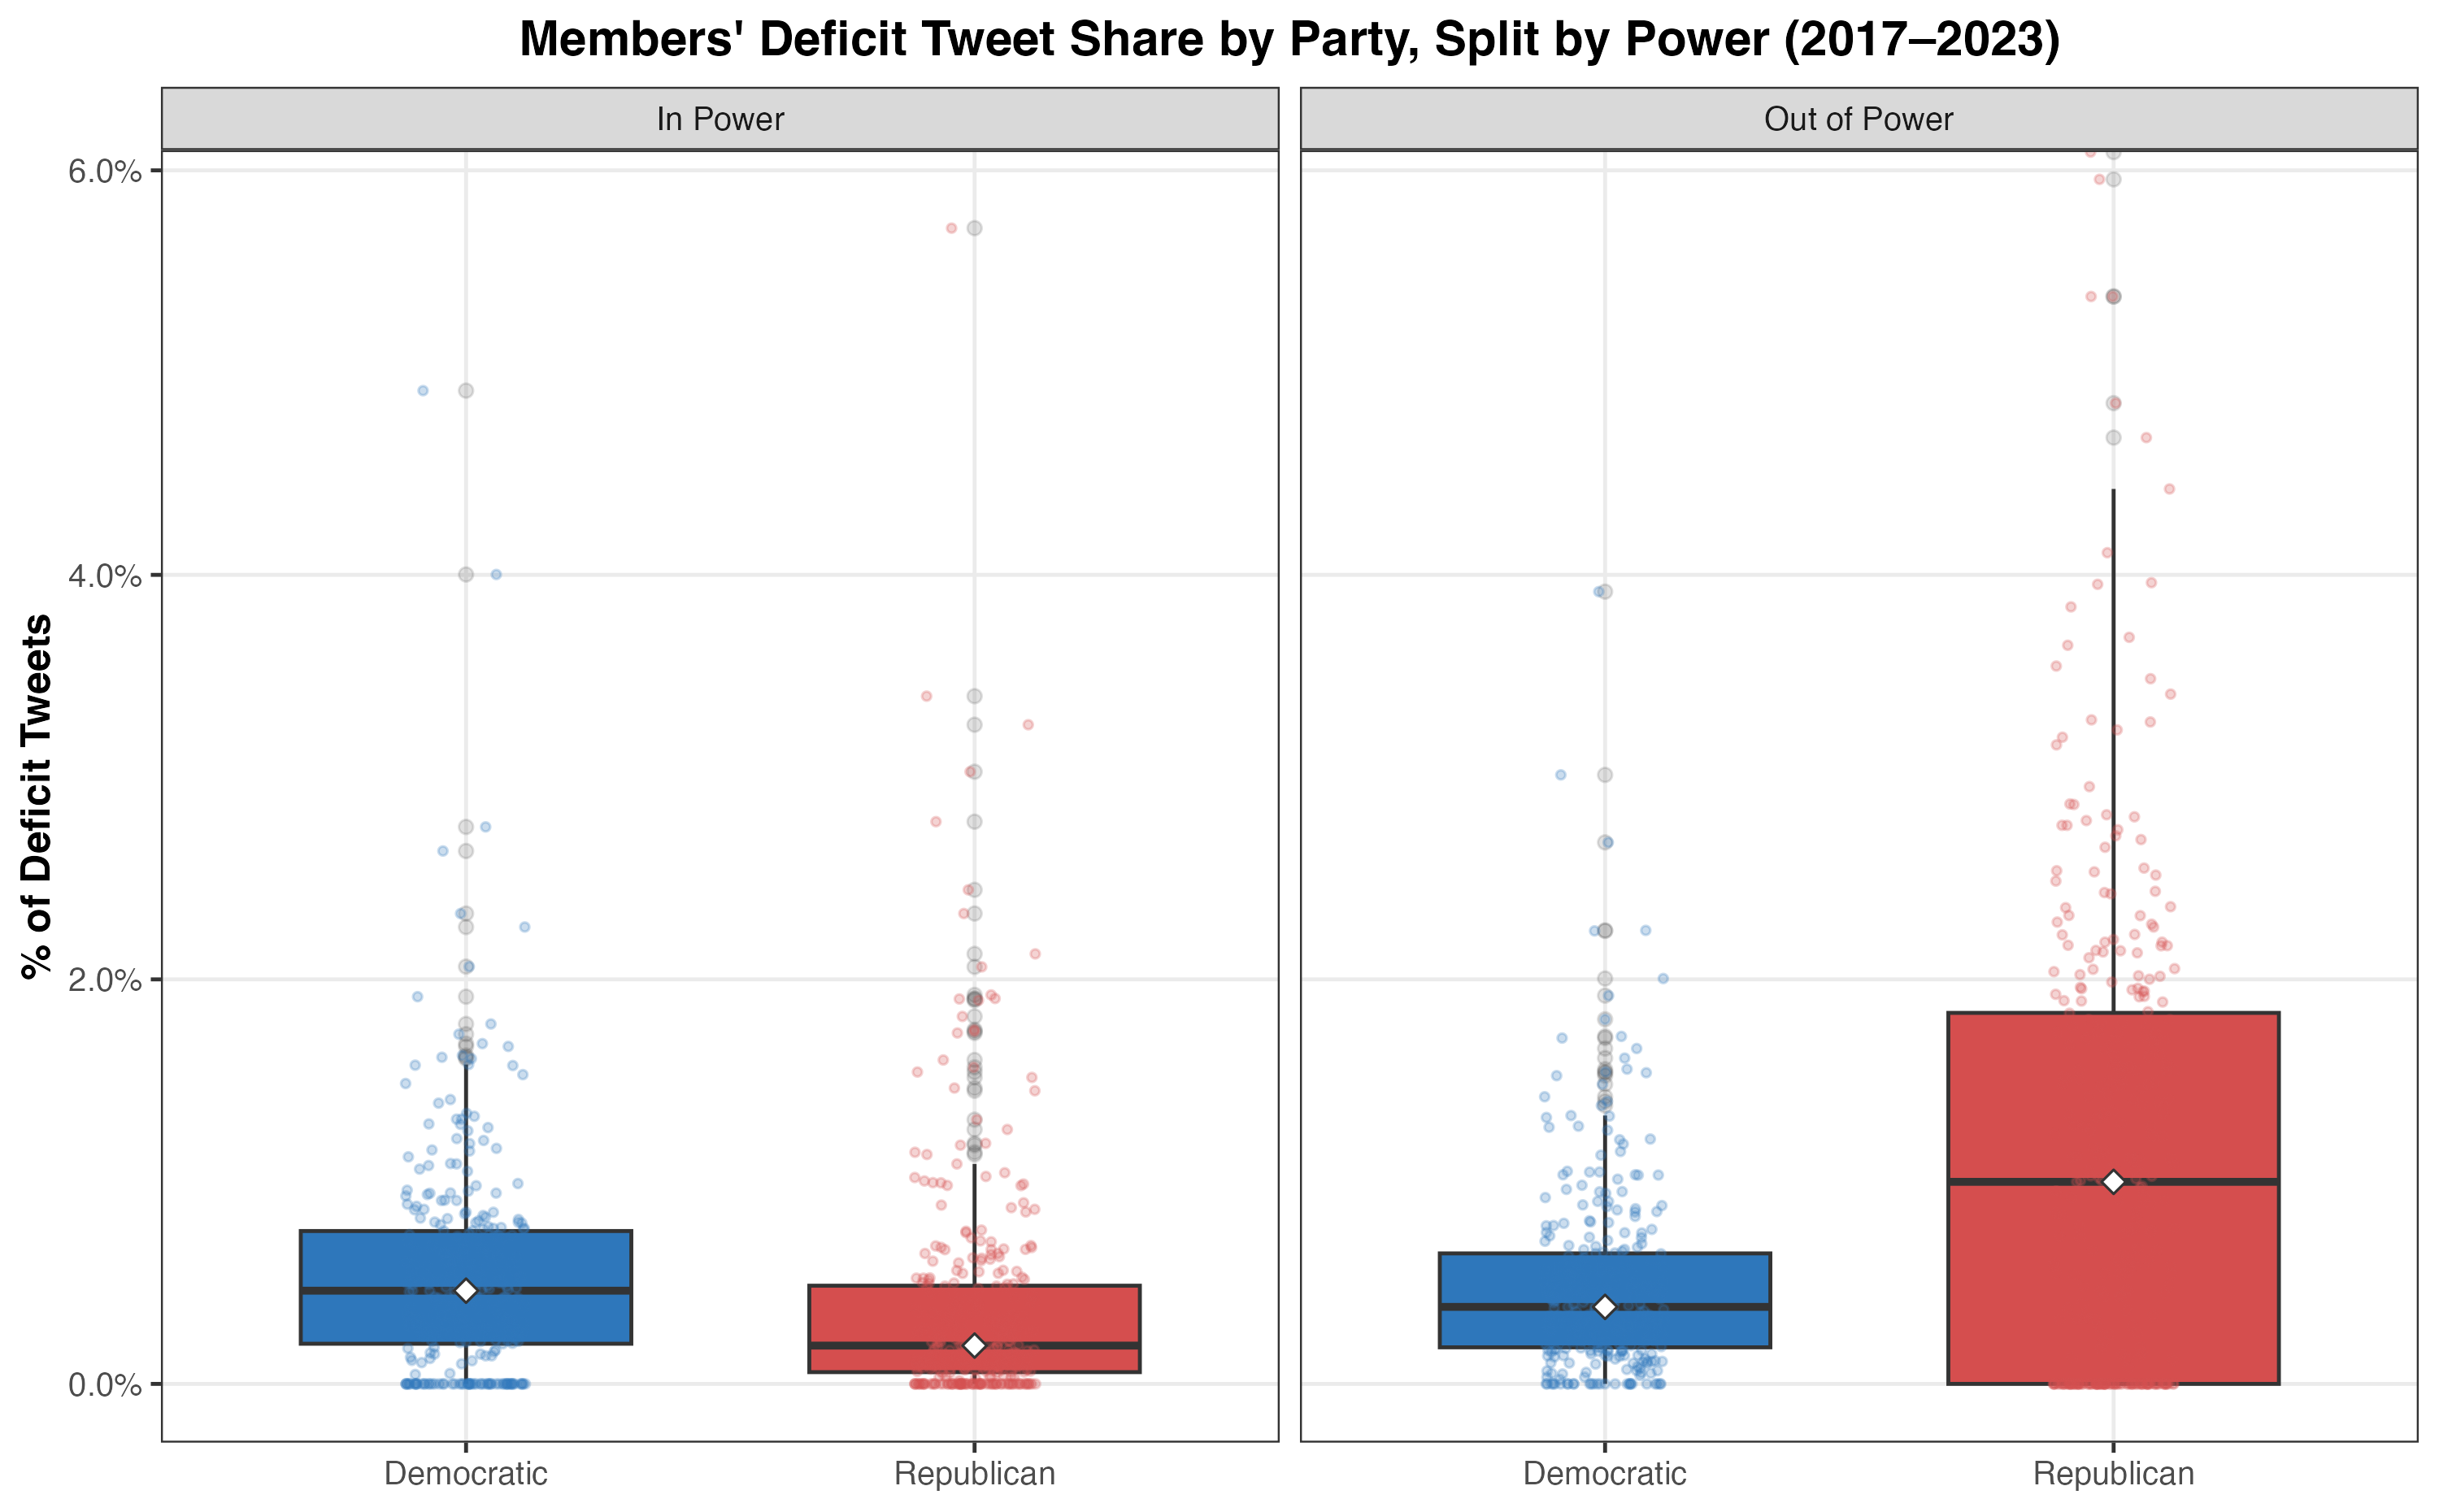
\includegraphics[width=0.85\textwidth,height=\textheight]{../figures/individuals/box_party_split_by_power.png}

}

\caption{\label{fig-power-boxplot}Distribution of deficit tweets by
power (boxplot).}

\end{figure}%

\begin{figure}

\centering{

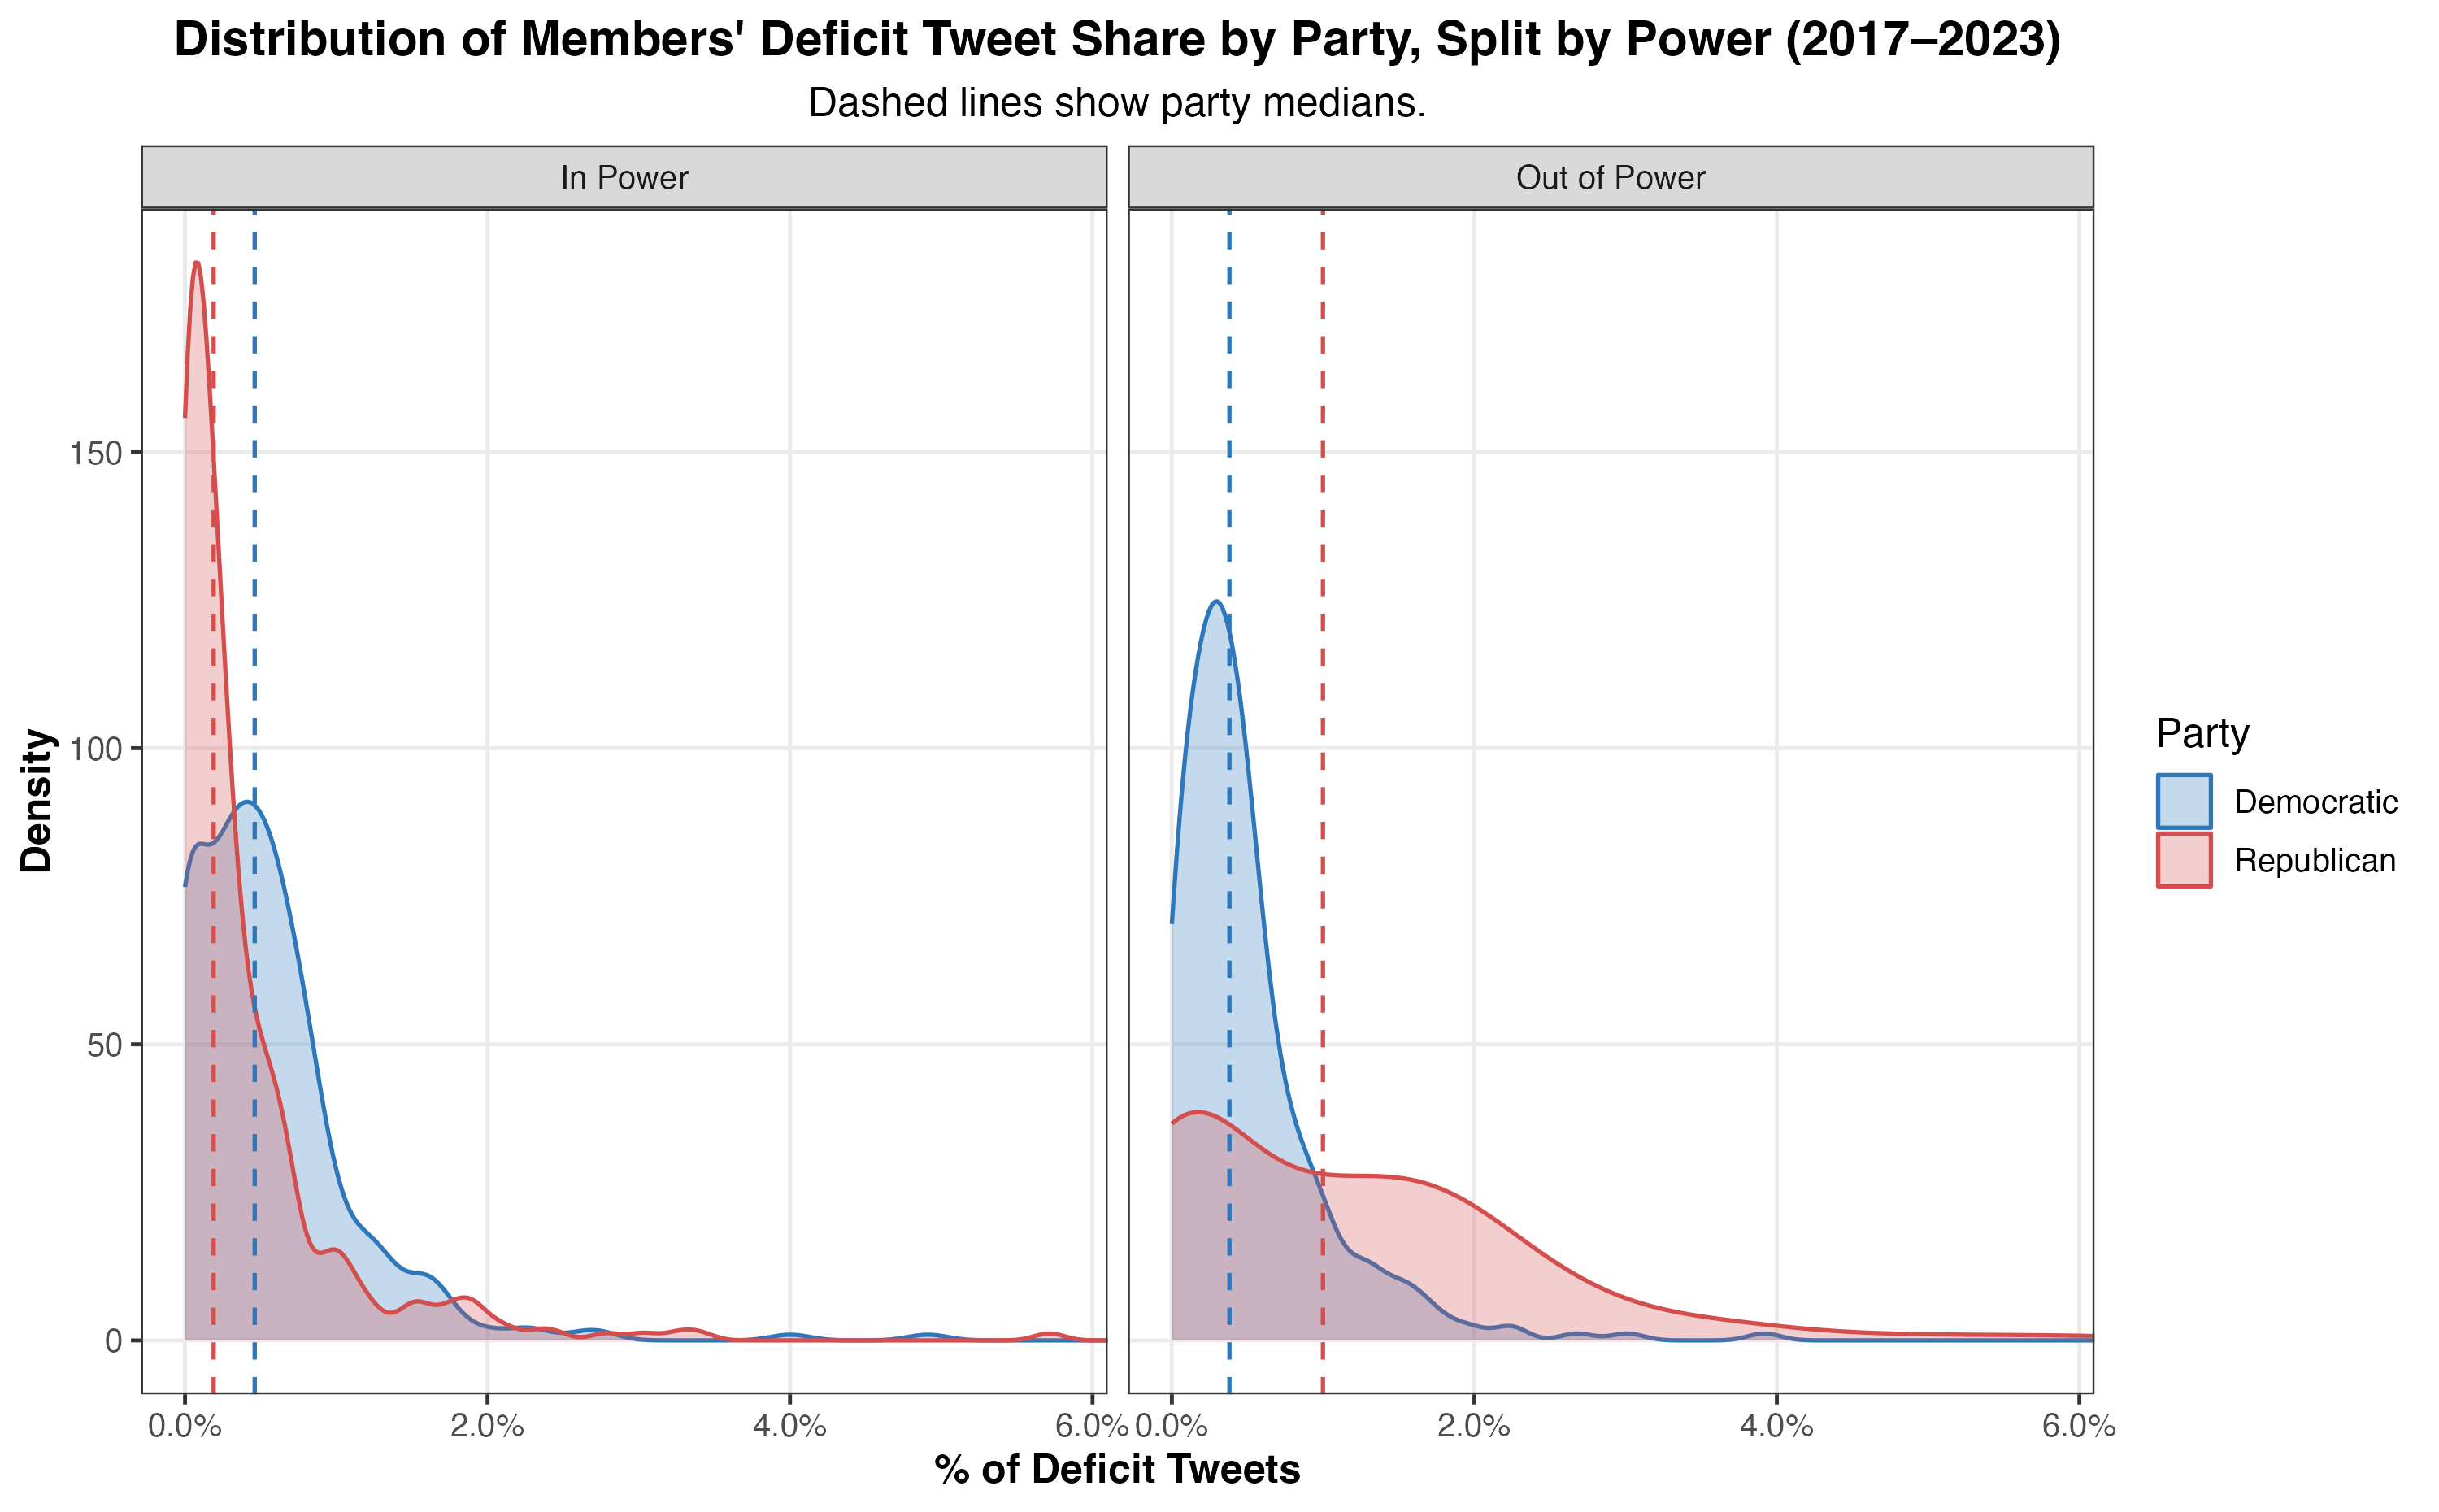
\includegraphics[width=0.85\textwidth,height=\textheight]{../figures/individuals/density_pct_deficit_by_party_split_power.png}

}

\caption{\label{fig-power-density}Distribution of deficit tweets by
power (density plot).}

\end{figure}%

\begin{figure}[H]

\centering{

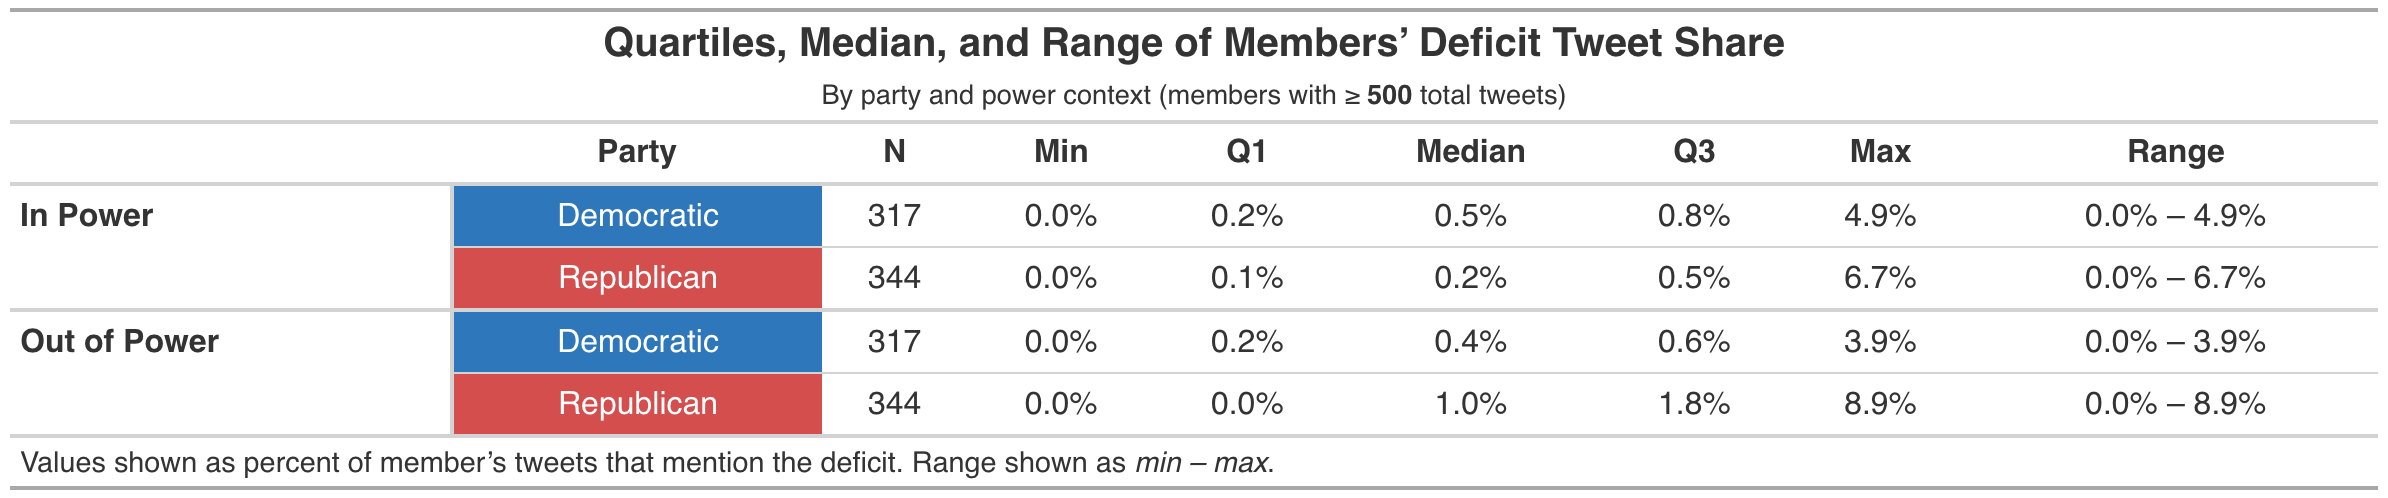
\includegraphics[width=0.75\textwidth,height=\textheight]{../figures/individuals/t_quartiles_by_party_power.png}

}

\caption{\label{fig-power-summary}Distribution of deficit tweets by
power (table).}

\end{figure}%

\FloatBarrier

As illustrated by the three figures above, Republicans' significant
right skew stems largely from their tweeting while out of power. For
instance, when moving between these contexts, the GOP median tweet share
increases five-fold \textbf{(0.2\% to 1.0\%)} and the inter-quartile
range from \textbf{(0.6\%)} to \textbf{(1.8\%)}. Democrats, by contrast,
remain relatively stable across contexts, with only a modest increase in
spread and averages when in power. \FloatBarrier

\begin{figure}

\centering{

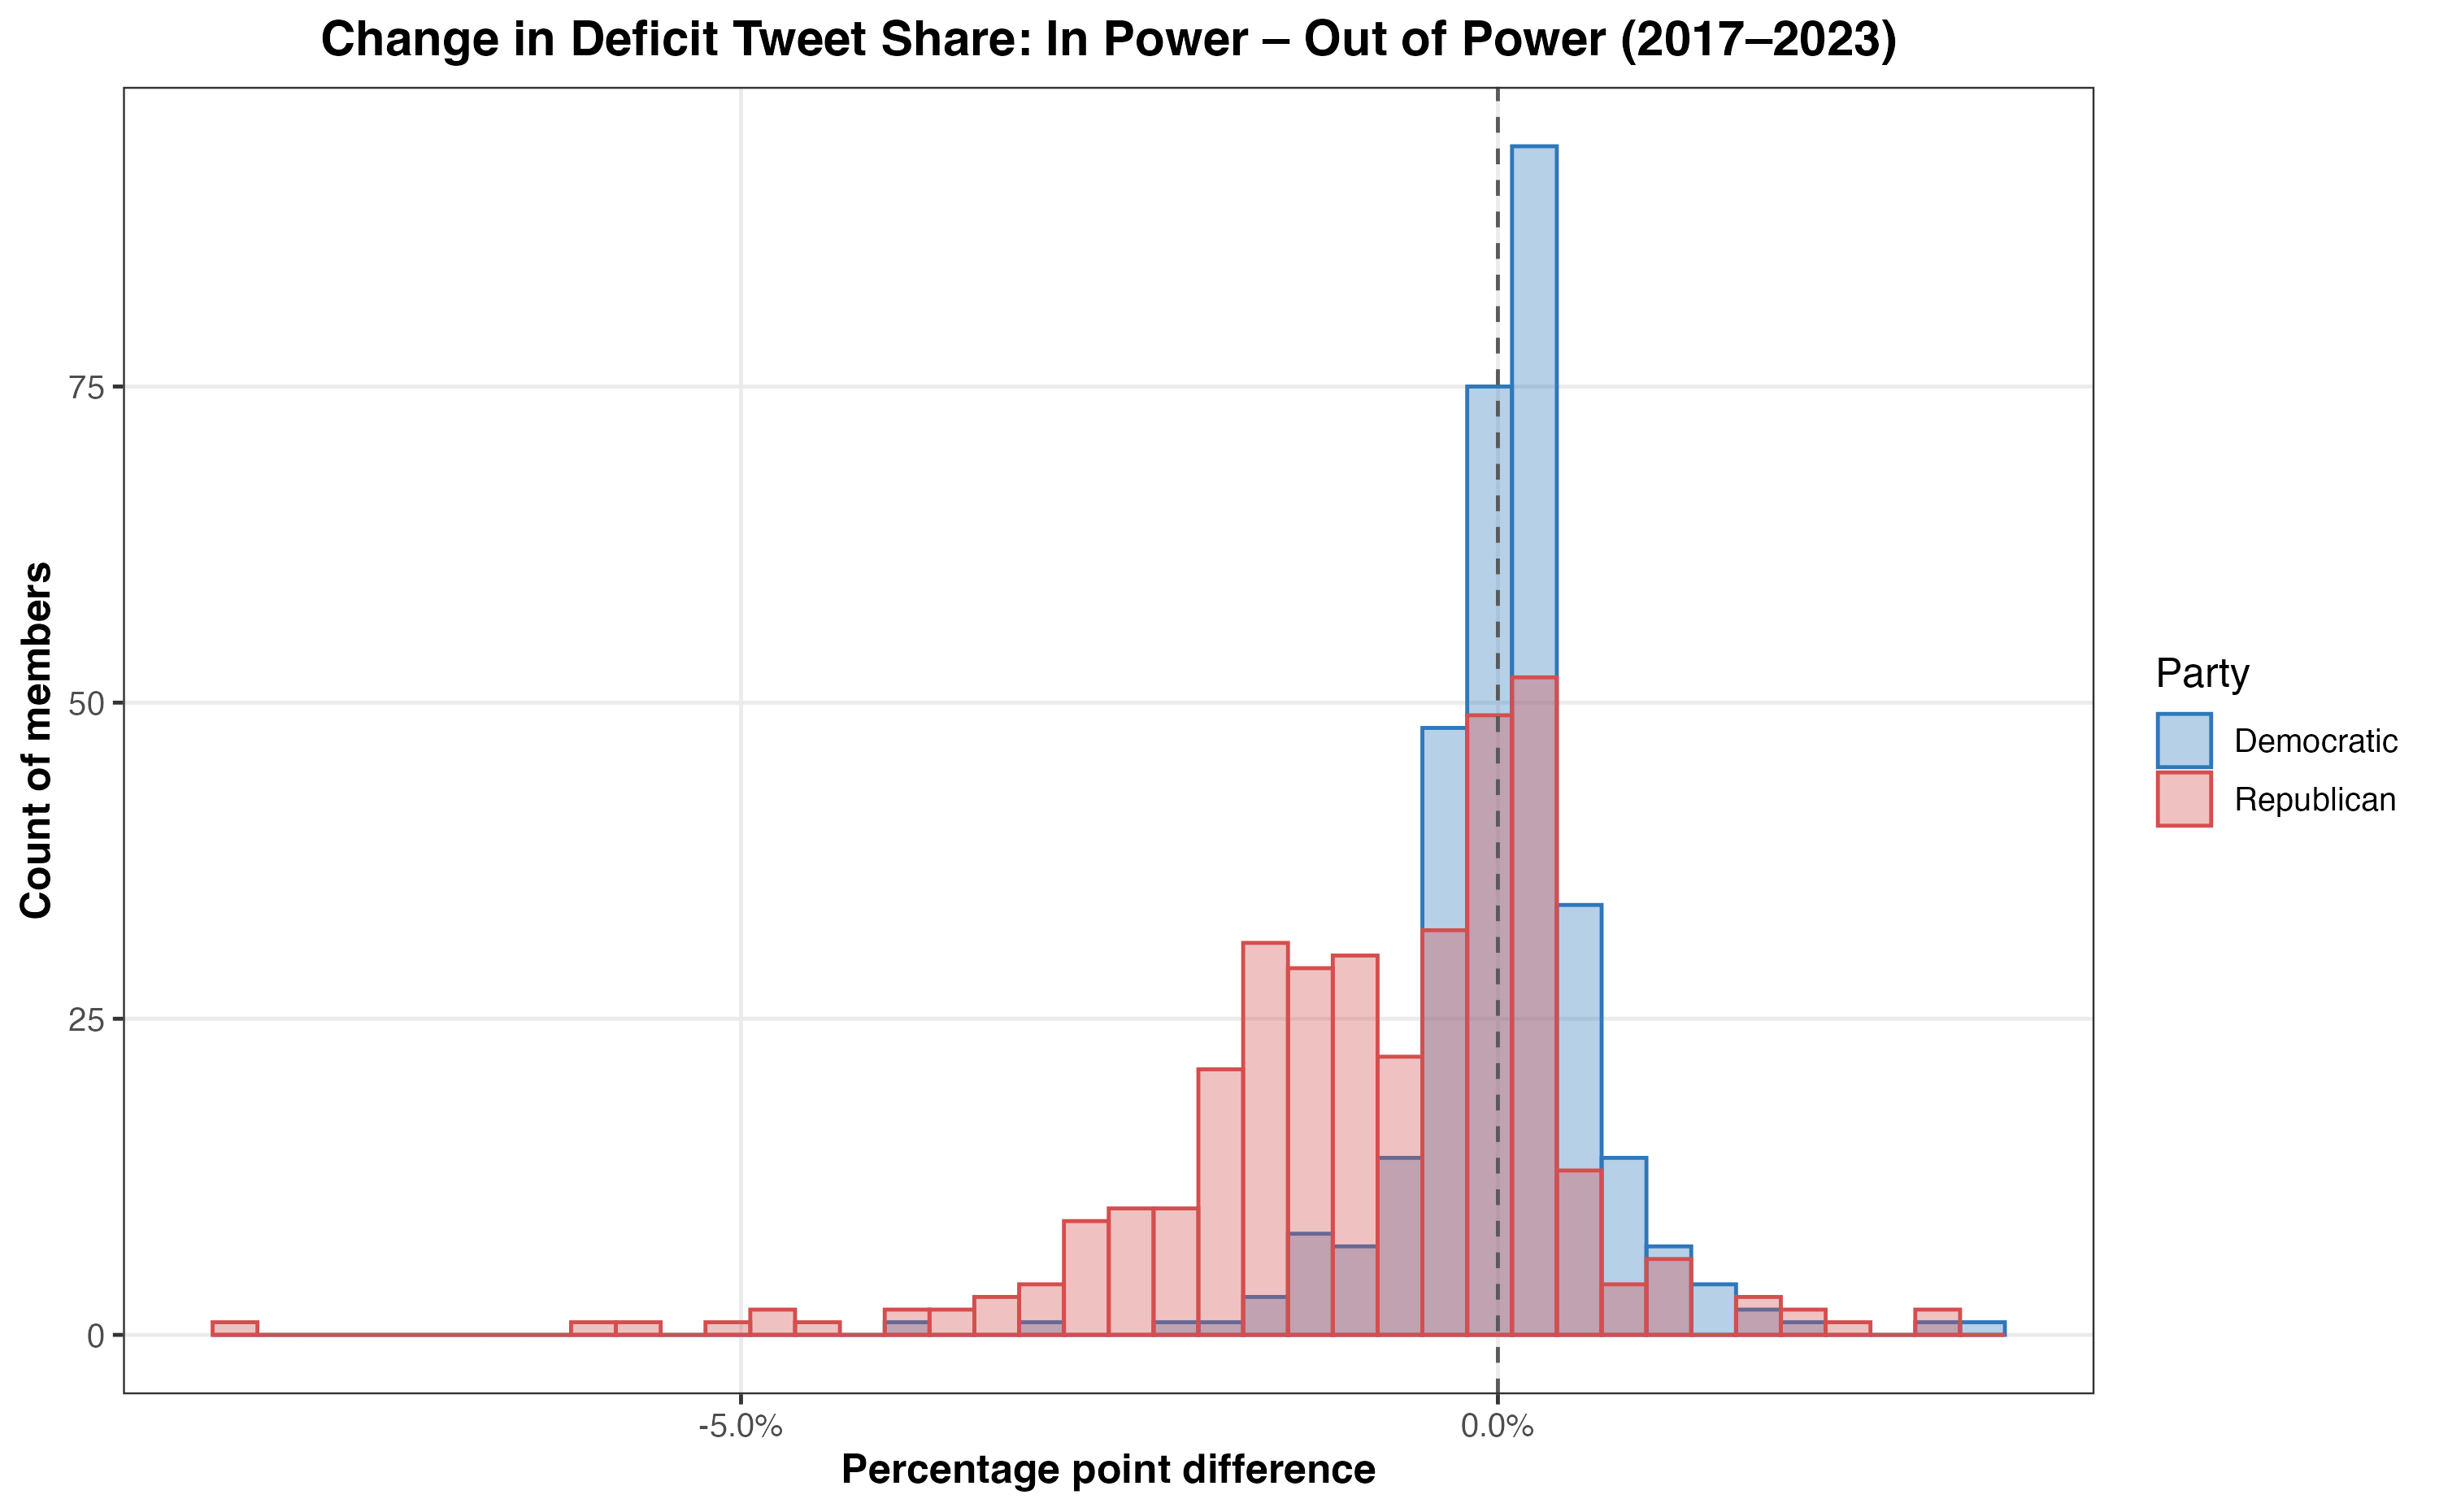
\includegraphics[width=0.85\textwidth,height=\textheight]{../figures/individuals/hist_in_minus_out_overlay.png}

}

\caption{\label{fig-inout-shifts}In--out shifts in deficit tweeting
(histogram).}

\end{figure}%

\begin{figure}[H]

\centering{

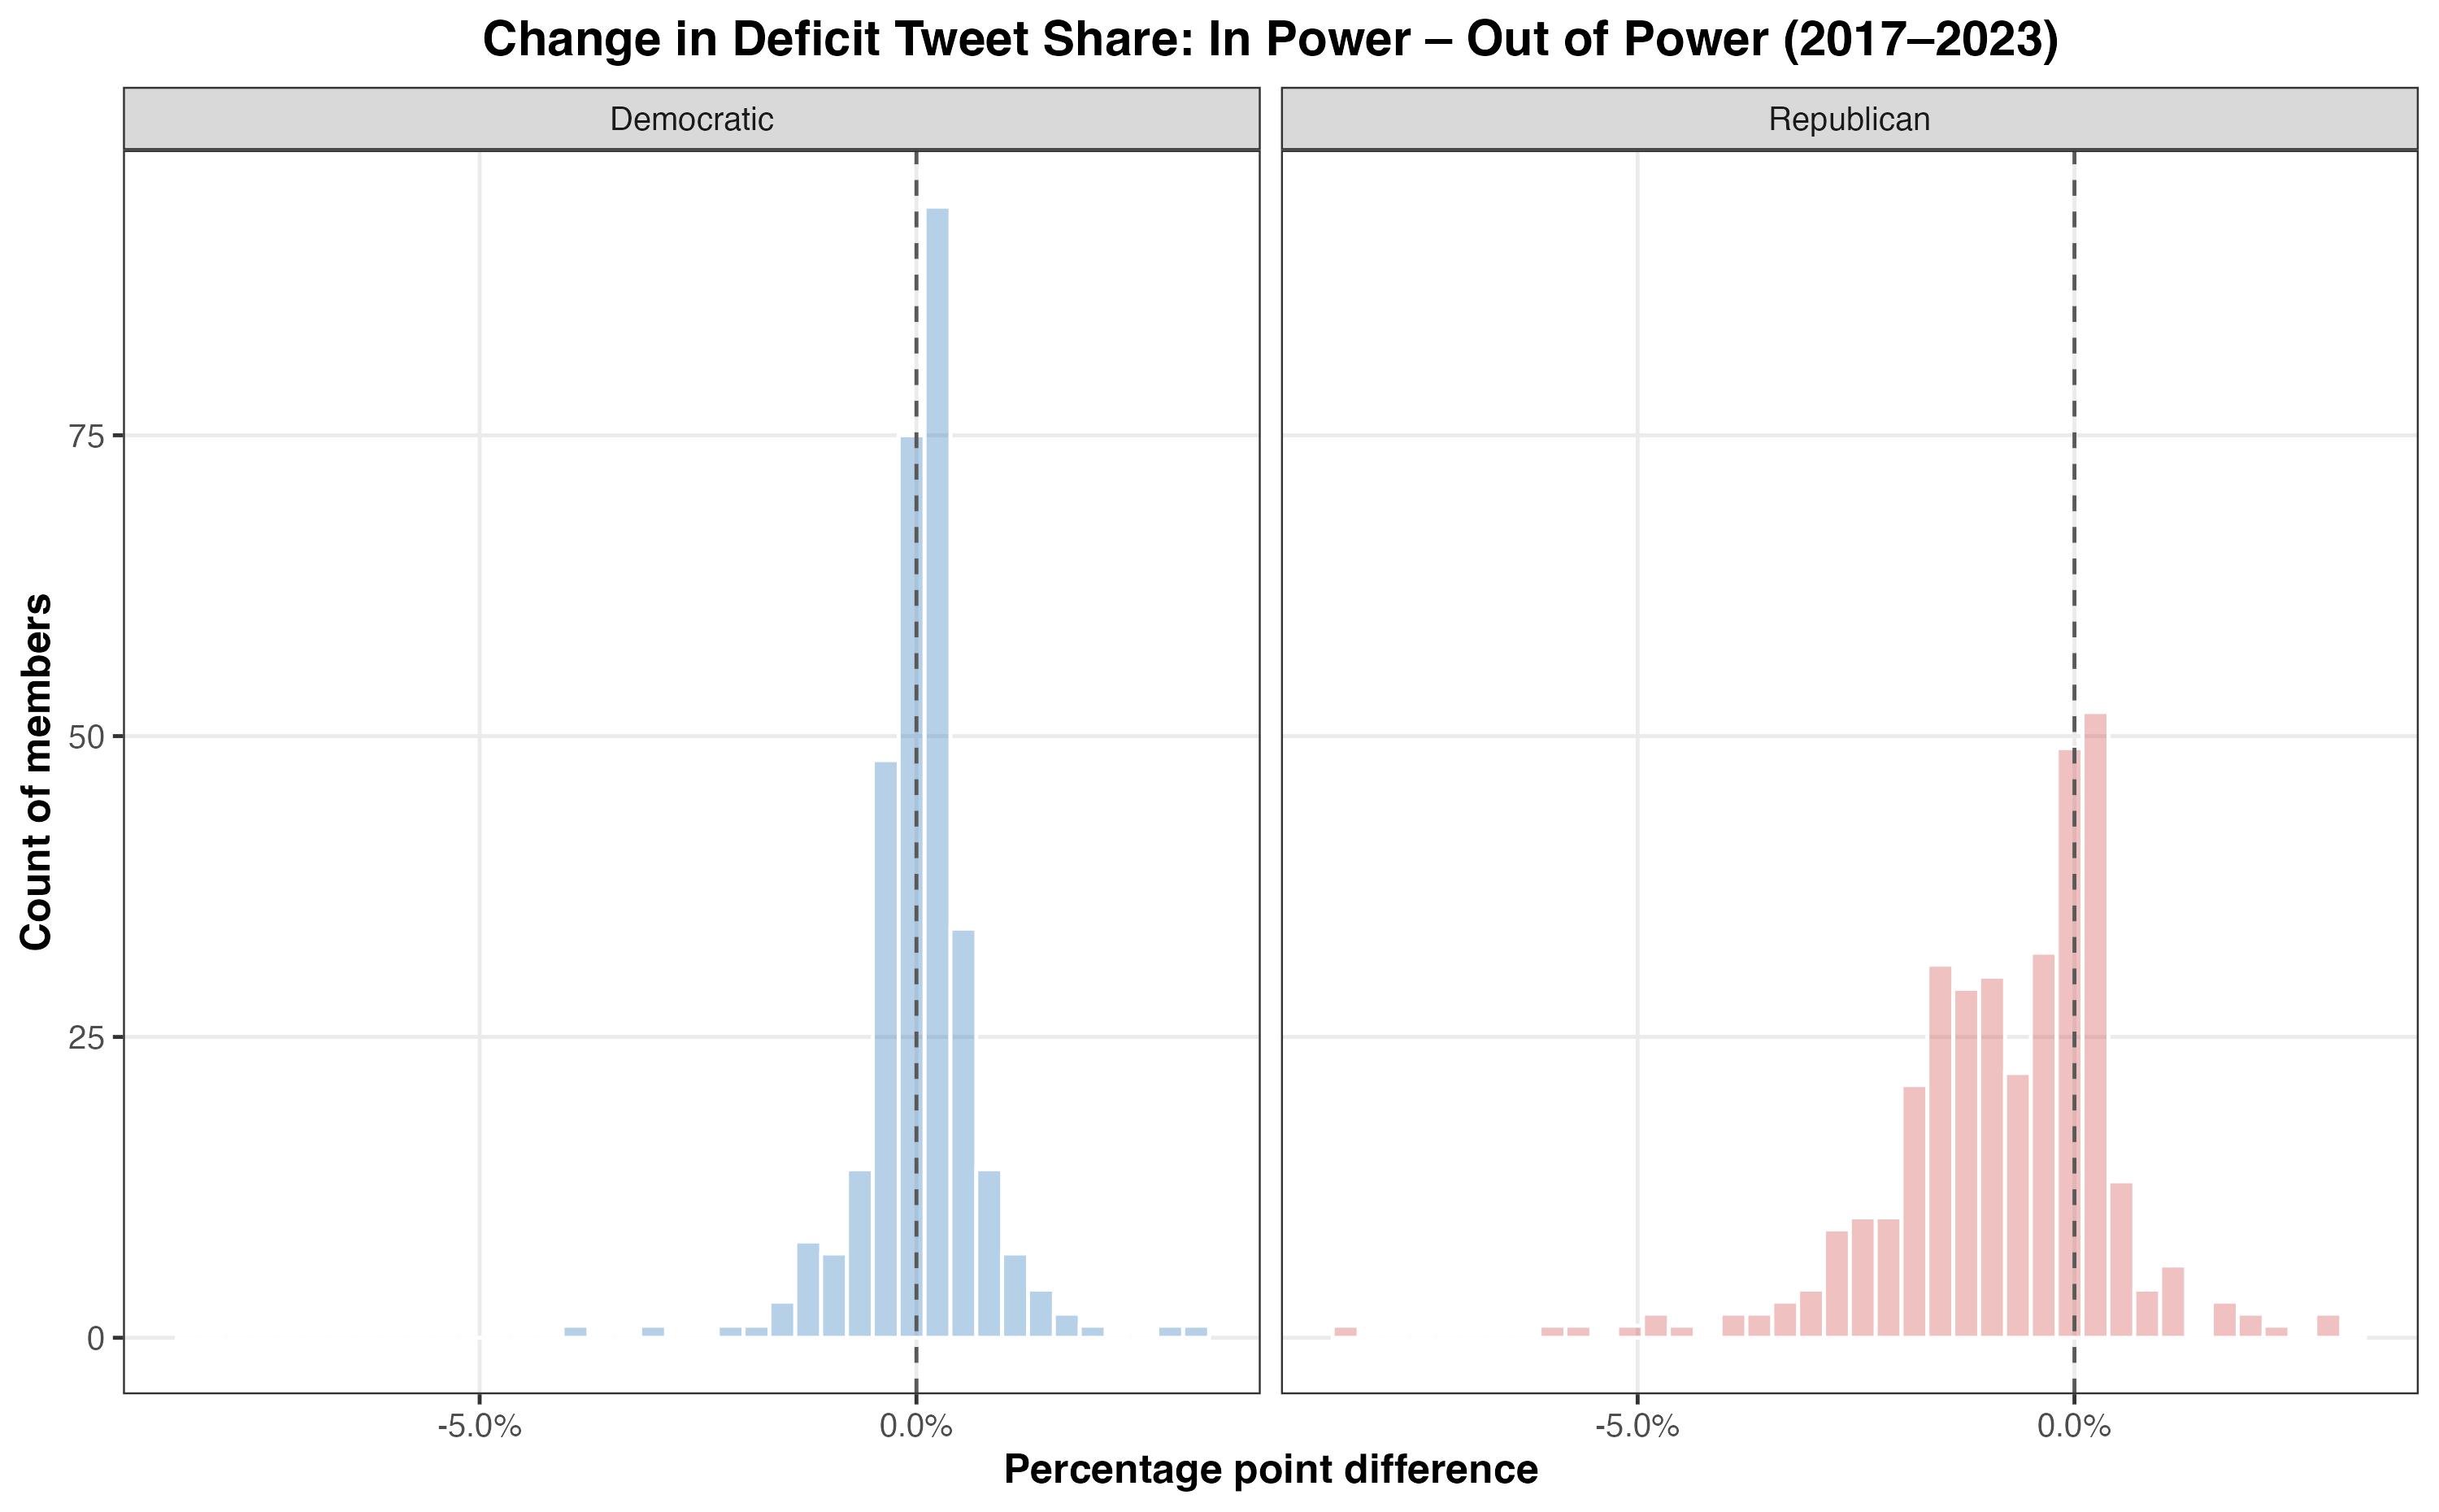
\includegraphics[width=0.75\textwidth,height=\textheight]{../figures/individuals/hist_in_minus_out_faceted.png}

}

\caption{\label{fig-inout-shifts-faceted}Faceted in--out shifts in
deficit tweeting (histograms by subgroup).}

\end{figure}%

\FloatBarrier

Histograms of the change in deficit tweeting further highlight these
asymmetries. Republicans' distribution is skewed negative, meaning the
party tweets at higher frequencies when out of power. Both figures
highlight this trend as the bulk of the GOP falls between
\textbf{(--5.0\%)} and \textbf{(+1\% )}. Democrats, however, are roughly
distributed around zero, indicating consistent levels of deficit
tweeting across power status contexts.

These distributions demonstrate three points. First, deficit tweeting is
relatively rare for both parties, with average levels rarely exceeding
\textbf{(+1.5\%)}. Second, most outliers -- the members who commit
\textbf{(4-8\%)} of their tweets to deficits -- are exclusively
Republicans. Third, the GOP systematically increases its tweet share
when out of power, whereas Democrats show little comparable shift.

\section{Leadership Analysis}\label{leadership-analysis}

\begin{figure}[H]

\centering{


\includegraphics[width=0.75\textwidth,height=\textheight]{../figures/leadership/leader_deficit_tweets.png}

}

\caption{\label{fig-leadership}Deficit tweeting by congressional leaders
(House and Senate; majority vs.~minority roles).}

\end{figure}%

\FloatBarrier

Figure~\ref{fig-leadership} summarizes deficit tweeting among House and
Senate leaders in both majority and minority roles. Tweeting patteerns
vary by party and institutional position, with the sharpest contrasts
appearing in the Senate. Senator Chuck Schumer tweeted about deficits
far more often as Majority Leader \textbf{(4.0\%)} than as Minority
Leader \textbf{(1.0\%)}, while Senator Mitch McConnell showed the
reverse, posting more in the minority \textbf{(1.9\%)} than the majority
\textbf{(0.05\%)}. Notably, in contrast to Seantor Schumer, her
Democratic counterpart, Representative Nancy Pelosi displayed higher
rates in the minority \textbf{(1.1\%)} than as Speaker \textbf{(0.5\%)}.
By comparison, Representatives Kevin McCarthy and Paul Ryan registered
very low shares overall, with McCarthy not posting a single
deficit-related tweet. \FloatBarrier

\section{Legislative Context}\label{legislative-context}

\begin{figure}[H]

\centering{


\includegraphics[width=0.75\textwidth,height=\textheight]{../results/tweetlevel_deficit_share_overall.png}

}

\caption{\label{fig-deficit-share-windows}Deficit share within
legislative windows.}

\end{figure}%

\begin{figure}[H]

\centering{


\includegraphics[width=0.75\textwidth,height=\textheight]{../results/tweetlevel_deficit_share_by_party.png}

}

\caption{\label{fig--deficit-share-by-party}Deficit share within
legislative windows, by party.}

\end{figure}%

\FloatBarrier

As noted, deficit tweeting is rare across Congress, with only
\textbf{(0.7\%)} of all tweets between 2017 and 2023 mentioning the
deficit Figure~\ref{fig-deficit-share-windows} . Legislative periods --
defined by one month before and after bill passage -- raise the
conditional rate modestly to \textbf{(0.9\%).} Industrial policy bills
-- the Inflation Reduction Act (IRA) and CHIPS Act, passed under
President Biden -- generated the highest levels of deficit tweeting
\textbf{(1.6\%)} among passed legislation. The Tax Cuts and Jobs Act
(2017), passed under President Trump, had a deficit tweet share of
\textbf{(1.2\%)} -- higher than baseline, but lower than the IRA/CHIPS.~

@fig--deficit-share-by-party decomposes these differences by party. At
baseline, Republicans tweet about the deficit more often
\textbf{(0.8\%)} than Democrats \textbf{(0.6\%)} -- a gap that persists
across most legislative windows. During the IRA and CHIPS periods,
Republicans' tweets accelerated, with deficit mentions at nearly
\textbf{(2.0\%)}, compared to \textbf{(1.3\%)} among Democrats. However,
the TCJA -- a partisan GOP tax cut-- is a noticeable and stark
exception. During these three months, the Democrats' deficit share
spikes to \textbf{(2.0\%)}, while the Republicans' share falls to just
\textbf{(0.2\%)}, reflecting a partisan realignment around a highly
divisive bill. In contrast, during the COVID relief period in 2020 -- a
non-partisan voting context -- both parties converged at very low levels
\textbf{(0.3--0.4\%)}.

\FloatBarrier

\section{Regression Visualization}\label{regression-visualization}

The following regression models offer a structured approach to examining
how institutional, fiscal, and partisan contexts affect the likelihood
of congressional deficit tweeting.

Since the specifications rely heavily on interaction terms, it is useful
to provide a framework for their interpretation first. The coefficients
are expressed as odds ratios: values above one indicate that Republicans
are more likely to tweet about deficits relative to Democrats. In
contrast, values below one indicate a narrowing of the GOP-Dem gap. Each
model includes majority interaction coefficients of the general form GOP
× Conditioning Variable. These coefficients indicate whether the
baseline Republican--Democratic difference changes under specific
conditions (legislative windows, presidential control, chamber control,
or trifectas).

\begin{figure}[H]

\centering{


\includegraphics[width=0.75\textwidth,height=\textheight]{../results/good_tables/r3_legislative_windows_main.png}

}

\caption{\label{fig-r1-legislative-windows}Regression 1: Legislative
windows.}

\end{figure}%

\FloatBarrier

The baseline model, Figure~\ref{fig-r1-legislative-windows}, examines
partisan differences in legislative periods without conditioning on
institutional control. The non-significant results suggest that, when
averaged across both Democratic and Republican presidencies, legislative
windows themselves do not systematically impact the partisan gap in
deficit tweeting.

\FloatBarrier

\begin{figure}[H]

\centering{


\includegraphics[width=0.75\textwidth,height=\textheight]{../results/good_tables/r5_majority_context_main.png}

}

\caption{\label{fig-r2-presidency}Regression 2: Majority context
(presidency).}

\end{figure}%

\FloatBarrier

Figure~\ref{fig-r2-presidency}, which controls for presidential party,
substantially changes the results from the preceding specification.

Republicans' odds of tweeting about deficits are nearly double
\textbf{(OR = 1.87)} when not holding the presidency compared to
Democrats under the same condition. In contrast, \textbf{GOP ×
Legislative window (OR = 0.38)} highlights that under a Republican
presidency, the partisan gap narrows during legislative months; the odds
of the GOP tweeting are \textbf{62\%} lower than those of Democrats.
This pattern aligns with Figure~\ref{fig-timeseries}, which shows that
Republican tweeting contracts while Democratic tweeting spikes as
Congress passes the Tax Cuts and Jobs Act in late 2017. However, the
three-way interaction coefficient \textbf{GOP × Legislative window ×
Minority presidency} reveals a reversal of this trend \textbf{(OR =
4.24)}. Under a Democratic presidency, Republicans' odds of tweeting are
more than four times higher than those of Democrats in the same
condition.

\FloatBarrier

\begin{figure}[H]

\centering{


\includegraphics[width=0.75\textwidth,height=\textheight]{../results/good_tables/r6_majority_context_combos.png}

}

\caption{\label{fig-r3-chamber-presidency}Regression 3: Majority context
--- chamber and presidency combinations.}

\end{figure}%

\FloatBarrier

The third model further examines the role of institutional power by
including combinations of chamber control. The regression baseline is
Democrats, outside legislative windows, when their party controls
nothing (i.e., a minority in the House and Senate; does not hold the
Presidency).

\textbf{GOP x Legislative window (OR = 0.31)} indicates that during
legislative months, when holding a trifecta, Republicans' odds of
tweeting are \textbf{69\%} lower than Democrats. The Tax Cuts and Jobs
Act (2017) -- a legislative window under a GOP trifecta -- is an
illustration of this circumstance. Once again, once we condition on a
Democratic trifecta, this effect reverses. Relative to the baseline
condition (a GOP trifecta), Republicans' odds of deficit tweeting are
seven times higher than those of Democrats in the same context. The
juxtaposition of these two coefficients \textbf{(OR = 0.31)} versus
\textbf{(OR = 7.00)} illustrates that legislative timing by itself isn't
determinative of tweeting gaps -- but who governs is. Under Democratic
control (i.e., 2021-2023), Republicans accelerate deficit rhetoric
during legislative months, while under the GOP trifecta (i.e.,
2017-2019), they significantly reduce deficit tweeting frequencies.

\subsection{\texorpdfstring{\textbf{Bill Partisanship and Fiscal
Magnitude}}{Bill Partisanship and Fiscal Magnitude}}\label{bill-partisanship-and-fiscal-magnitude}

Across all three specifications, the coefficients for Fiscal magnitude
(z) remain consistently insignificant (\textasciitilde1.0).~ These
coefficients, based on a normalized measure of a given bill's 10-year
CBO estimate, suggest that the fiscal consequences of policy do not
systematically impact partisan tweeting gaps.

Bill partisanship (z), however, shows significant contractions in the
GOP-Dem tweeting gap once institutional control is included \textbf{(OR
\textasciitilde{} 0.50)}. In other words, for each one-SD increase in a
bill's partisanship score, the GOP-Dem gap contracts by roughly half.
Notably, because these variables are continuous (ie, z-scores), the
coefficients represent slopes rather than a baseline-specific effect.
For example, in the context of bill partisanship, if Republicans are
twice as likely as Democrats to tweet at \textbf{z = 0 (OR = 2.0)}, that
gap narrows to parity at \textbf{z = 1 (OR = 1.0).}

\FloatBarrier




\end{document}
